% ============================================================
\chapter{ARIMA Models and Differencing}
\label{ch:arima}
% ============================================================

\section{Motivating example}
The French quarterly GDP exhibits an upward trend: it is not stationary. After differencing ($\nabla X_t = X_t - X_{t-1}$), the growth rate is approximately stationary and can be modelled by an ARMA process.

\section{Integrated processes}\index{integrated process}

\begin{definition}[Integrated process of order $d$]
$(X_t)$ is \textbf{integrated of order $d$}, denoted $X_t\sim I(d)$, if $\nabla^d X_t = (1-B)^d X_t$ is stationary but $\nabla^{d-1}X_t$ is not.
\end{definition}

\begin{example}
The random walk $X_t=X_{t-1}+\eps_t$ is $I(1)$ since $\nabla X_t = \eps_t$ is stationary.
\end{example}

\section{ARIMA$(p,d,q)$ model}\index{ARIMA}

\begin{definition}[ARIMA$(p,d,q)$]
\[
\phi(B)(1-B)^d X_t = \theta(B)\eps_t.
\]
$X_t$ follows an ARIMA$(p,d,q)$ if $W_t = \nabla^d X_t$ follows an ARMA$(p,q)$.
\end{definition}

\begin{warning}
One differences to achieve stationarity, but \textbf{over-differencing} ($d$ too large) introduces MA roots close to the unit circle, which degrades forecasts. In practice, $d\leq 2$.
\end{warning}

\section{SARIMA: seasonality}\index{SARIMA}

\begin{definition}[SARIMA$(p,d,q)\times(P,D,Q)_s$]
For a series with period $s$:
\[
\Phi(B^s)\phi(B)(1-B)^d(1-B^s)^D X_t = \Theta(B^s)\theta(B)\eps_t,
\]
where $\Phi$, $\Theta$ are the seasonal polynomials of orders $P$, $Q$.
\end{definition}

\begin{example}[Airline model]
The Box--Jenkins model for AirPassengers is a SARIMA$(0,1,1)\times(0,1,1)_{12}$:
\[
(1-B)(1-B^{12})X_t = (1+\theta_1 B)(1+\Theta_1 B^{12})\eps_t.
\]
\end{example}

\section{Differencing strategy}

\begin{method}
\begin{enumerate}
\item Plot the series and its ACF. If the ACF decays very slowly, difference.
\item Apply the ADF test (or KPSS). If $H_0$ (unit root) is not rejected, difference.
\item After differencing, verify that the resulting series is stationary.
\item For seasonality, difference at order $s$ if the ACF shows periodic peaks.
\end{enumerate}
\end{method}

\section{Numerical example: AirPassengers}

\begin{center}
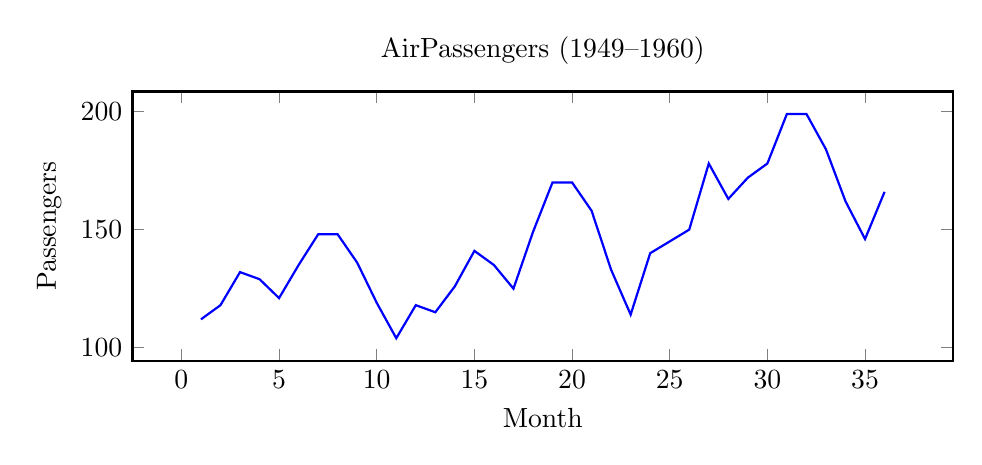
\begin{tikzpicture}
\begin{axis}[
  width=12cm, height=5cm, xlabel={Month}, ylabel={Passengers},
  title={AirPassengers (1949--1960)}, no markers, thick
]
\addplot[blue] coordinates {
(1,112)(2,118)(3,132)(4,129)(5,121)(6,135)(7,148)(8,148)(9,136)
(10,119)(11,104)(12,118)(13,115)(14,126)(15,141)(16,135)(17,125)
(18,149)(19,170)(20,170)(21,158)(22,133)(23,114)(24,140)
(25,145)(26,150)(27,178)(28,163)(29,172)(30,178)(31,199)(32,199)
(33,184)(34,162)(35,146)(36,166)
};
\end{axis}
\end{tikzpicture}
\end{center}

\section{Implementation}

\begin{codeblock}[title=\textbf{Python}]
\begin{minted}{python}
import numpy as np
import pandas as pd
import matplotlib.pyplot as plt
from statsmodels.tsa.arima.model import ARIMA
from statsmodels.tsa.statespace.sarimax import SARIMAX
from statsmodels.tsa.stattools import adfuller
from statsmodels.graphics.tsaplots import plot_acf, plot_pacf
import pmdarima as pm

# Charger AirPassengers
url = ('https://raw.githubusercontent.com/jbrownlee/Datasets/'
       'master/airline-passengers.csv')
df = pd.read_csv(url, parse_dates=['Month'], index_col='Month')
y = df['Passengers']

# Log-transformation (stabilise la variance)
y_log = np.log(y)

# Test ADF
print("ADF sur log(y):", adfuller(y_log)[1])  # > 0.05 => non stat.
y_diff = y_log.diff().dropna()
print("ADF sur diff(log(y)):", adfuller(y_diff)[1])  # < 0.05 => stat.

# SARIMA automatique
auto_model = pm.auto_arima(y_log, seasonal=True, m=12,
                           stepwise=True, trace=True)
print(auto_model.summary())

# Ajustement SARIMA(0,1,1)(0,1,1)[12]
model = SARIMAX(y_log, order=(0,1,1),
                seasonal_order=(0,1,1,12))
results = model.fit(disp=False)
print(results.summary())

# Prévision
forecast = results.get_forecast(steps=24)
pred = np.exp(forecast.predicted_mean)
ci = np.exp(forecast.conf_int())

fig, ax = plt.subplots(figsize=(12, 5))
y.plot(ax=ax, label='Observé')
pred.plot(ax=ax, label='Prévision', color='red')
ax.fill_between(ci.index, ci.iloc[:,0], ci.iloc[:,1],
                alpha=0.2, color='red')
ax.legend()
ax.set_title('SARIMA — AirPassengers')
plt.savefig('ch05_arima.pdf')
plt.show()
\end{minted}
\end{codeblock}

\section{Exercises}

\begin{exercise}[$\star$]
Show that $(1-B)^2 X_t = X_t - 2X_{t-1}+X_{t-2}$.
\end{exercise}

\begin{exercise}[$\star$]
Apply \texttt{pm.auto\_arima} to a series of your choice. Interpret the selected model.
\end{exercise}

\begin{exercise}[$\star\star$]
Show that if $X_t\sim\text{ARIMA}(p,1,q)$, then the long-term forecasts converge to a straight line (constant forecast in differenced levels).
\end{exercise}

\begin{exercise}[$\star\star\star$ -- Project]
Model the quarterly GDP of a country using a seasonal ARIMA. Compare out-of-sample forecasts with different orders.
\end{exercise}

\begin{keyformulas}
\begin{align*}
\text{ARIMA}(p,d,q) &: \phi(B)(1-B)^d X_t = \theta(B)\eps_t \\
\text{SARIMA} &: \Phi(B^s)\phi(B)(1-B)^d(1-B^s)^D X_t = \Theta(B^s)\theta(B)\eps_t \\
I(d) &: \nabla^d X_t\text{ stationary}, \nabla^{d-1}X_t\text{ not}
\end{align*}
\end{keyformulas}
